%%%%%%%%%%%%%%%%%%%%%%%%%%%%% Define Article %%%%%%%%%%%%%%%%%%%%%%%%%%%%%%%%%%
\documentclass{article}   % two side printing
%%%%%%%%%%%%%%%%%%%%%%%%%%%%%%%%%%%%%%%%%%%%%%%%%%%%%%%%%%%%%%%%%%%%%%%%%%%%%%%

%%%%%%%%%%%%%%%%%%%%%%%%%%%%% Using Packages %%%%%%%%%%%%%%%%%%%%%%%%%%%%%%%%%%
\usepackage{geometry}
\usepackage{graphicx}
\usepackage{amssymb}
\usepackage{amsmath}
\usepackage{amsthm}
\usepackage{empheq}
\usepackage{mdframed}
\usepackage{booktabs}
\usepackage{lipsum}
\usepackage{color}
\usepackage{psfrag}
\usepackage{pgfplots}   % For plotting beautiful graphs
\usepackage{bm}
\usepackage[spanish]{babel}
\usepackage{biblatex} 
\usepackage{csquotes} 
\usepackage{setspace}
\usepackage{multicol}  
\usepackage[skip=3pt plus 1pt, indent=30pt]{parskip}    % Setting space between paragraphs and indent
\usepackage[T1]{fontenc}    % Output font encoding for international characters
\usepackage{helvet}        % Selecting font family
\usepackage{ragged2e}      % For text alignment
\usepackage{adjustbox}       % For defining new environments
\usepackage{fancyhdr}       % For defining headers and footers
\usepackage[cochineal]{newtxmath}
\usepackage{caption}
\usetikzlibrary{intersections}
\usetikzlibrary{decorations.text}
\usetikzlibrary{decorations.pathreplacing}
%%%%%%%%%%%%%%%%%%%%%%%%%%%%%%%%%%%%%%%%%%%%%%%%%%%%%%%%%%%%%%%%%%%%%%%%%%%%%%%

% Other Settings
\newcommand*{\freq}{\mathord{\mathit{f}}}
%\let\cleardoublepage=\clearpage
%\renewcommand{\baselinestretch}{1.5}
%%%%%%%%%%%%%%%%%%%%%%%%%% Page Setting %%%%%%%%%%%%%%%%%%%%%%%%%%%%%%%%%%%%%%%
\geometry{a4paper, textwidth=19cm, textheight=28.5cm, top=0.1cm, headheight=0.1cm}  % Setting page size
\graphicspath{{images/}}    % Setting path for images
\addbibresource{bibliography.bib}   % Setting path for bibliography
%%%%%%%%%%%%%%%%%%%%%%%%%% Define some useful colors %%%%%%%%%%%%%%%%%%%%%%%%%%
\definecolor{ocre}{RGB}{243,102,25}
\definecolor{mygray}{RGB}{243,243,244}
\definecolor{deepGreen}{RGB}{26,111,0}
\definecolor{shallowGreen}{RGB}{235,255,255}
\definecolor{deepBlue}{RGB}{61,124,222}
\definecolor{shallowBlue}{RGB}{235,249,255}
%%%%%%%%%%%%%%%%%%%%%%%%%%%%%%%%%%%%%%%%%%%%%%%%%%%%%%%%%%%%%%%%%%%%%%%%%%%%%%%

%%%%%%%%%%%%%%%%%%%%%%%%%% Define an orange box command %%%%%%%%%%%%%%%%%%%%%%%%
\newcommand\orangebox[1]{\fcolorbox{ocre}{mygray}{\hspace{1em}#1\hspace{1em}}}
%%%%%%%%%%%%%%%%%%%%%%%%%%%%%%%%%%%%%%%%%%%%%%%%%%%%%%%%%%%%%%%%%%%%%%%%%%%%%%%

%%%%%%%%%%%%%%%%%%%%%%%%%%%% English Environments %%%%%%%%%%%%%%%%%%%%%%%%%%%%%
\newtheoremstyle{mytheoremstyle}{3pt}{3pt}{\normalfont}{0cm}{\rmfamily\bfseries}{}{1em}{{\color{black}\thmname{#1}~\thmnumber{#2}}\thmnote{\,--\,#3}}
\newtheoremstyle{myproblemstyle}{3pt}{3pt}{\normalfont}{0cm}{\rmfamily\bfseries}{}{1em}{{\color{black}\thmname{#1}~\thmnumber{#2}}\thmnote{\,--\,#3}}
\theoremstyle{mytheoremstyle}
\newmdtheoremenv[linewidth=1pt,backgroundcolor=shallowGreen,linecolor=deepGreen,leftmargin=0pt,innerleftmargin=20pt,innerrightmargin=20pt,]{theorem}{Theorem}[section]
\theoremstyle{mytheoremstyle}
\newmdtheoremenv[linewidth=1pt,backgroundcolor=shallowBlue,linecolor=deepBlue,leftmargin=0pt,innerleftmargin=20pt,innerrightmargin=20pt,]{definition}{Definition}[section]
\theoremstyle{myproblemstyle}
\newmdtheoremenv[linecolor=black,leftmargin=0pt,innerleftmargin=10pt,innerrightmargin=10pt,]{problem}{Problem}[section]
%%%%%%%%%%%%%%%%%%%%%%%%%%%%%%%%%%%%%%%%%%%%%%%%%%%%%%%%%%%%%%%%%%%%%%%%%%%%%%%

%%%%%%%%%%%%%%%%%%%%%%%%%%%%%%% Plotting Settings %%%%%%%%%%%%%%%%%%%%%%%%%%%%%
\usepgfplotslibrary{colorbrewer}
\pgfplotsset{width=8cm,compat=1.9}
%%%%%%%%%%%%%%%%%%%%%%%%%%%%%%%%%%%%%%%%%%%%%%%%%%%%%%%%%%%%%%%%%%%%%%%%%%%%%%%

%%%%%%%%%%%%%%%%%%%%%%%%%%%%%%% Title & Author %%%%%%%%%%%%%%%%%%%%%%%%%%%%%%%%
\title{Análisis de lineas de transmisión utilizando el Diagrama de Schmidt}
\author{Luis Guillermo Macias Rojas}
%%%%%%%%%%%%%%%%%%%%%%%%%%%%%%%%%%%%%%%%%%%%%%%%%%%%%%%%%%%%%%%%%%%%%%%%%%%%%%%

%%%%%%%%%%%%%%%%%%%%%%%%%%%%%%% Header & Footer %%%%%%%%%%%%%%%%%%%%%%%%%%%%%%%
\pagestyle{fancy}  % Setting page style
\fancyhf{}
\fancyhead[L]{\text{Luis Guillermo Macias Rojas}}  % Setting header
%%%%%%%%%%%%%%%%%%%%%%%%%%%%%%%%%%%%%%%%%%%%%%%%%%%%%%%%%%%%%%%%%%%%%%%%%%%%%%%

\begin{document}
    \maketitle

    \fontfamily{phv}\selectfont % Selecting font family
    \noindent
    \textbf{Resumen:} Este estudio exploró el comportamiento de cinco condiciones de carga en líneas de transmisión ($Z_0$) 
    utilizando el Diagrama de Schmidt, con el objetivo de correlacionar la ubicación de impedancias normalizadas ($z = \frac{Z_L}{Z_0}$)
    con el coeficiente de reflexión ($\Gamma$). Los casos analizados incluyeron: cortocircuito ($Z_L = 0$), circuito abierto 
    ($Z_L \to \infty$), acoplamiento perfecto ($Z_L = Z_0$), y cargas resistivas con $Z_L > Z_0$ y $Z_L < Z_0$. El análisis
    reveló que la posición de $\Gamma$ en el diagrama indica la relación entre $Z_{ref}$ y $Z_0$, mientras que el radio de la circunferencia
    indica la magnitud de la reflexión (determinada por la relación entre $Z_L$ y $Z_0$).

    \noindent\begin{minipage}{0.49\textwidth}   %uses 60% of the page
        {\centering\section*{\large Introducción}}

        El Diagrama de Schmidt es una herramienta gráfica fundamental en el diseño y análisis de circuitos de microondas, 
        especialmente para trabajar con líneas de transmisión y problemas de acoplamiento de impedancias. Este diagrama permite 
        visualizar y resolver de manera intuitiva relaciones complejas entre impedancias (o admitancias), coeficientes de 
        reflexión ($\Gamma$) y parámetros de líneas de transmisión, evitando cálculos matemáticos extensos. $\Gamma$ determina
        la pérdida por retorno de una línea de transmisión, que es la proporción de la onda reflejada respecto a la onda
        incidente y está determinanado por la impedancia de carga ($Z_L$) y la impedancia característica de la línea ($Z_0$) 
        mediante la ecuacion \eqref{eq:gamma}.

        \begin{equation}
            \Gamma = \frac{Z_L-Z_0}{Z_L+Z_0}
            \label{eq:gamma}
        \end{equation}
        
        La posición de $\Gamma$ en el diagrama indica si la carga está acoplada ($\Gamma$=0), cortocircuitada ($\Gamma$=-1),
        o en circuito abierto ($\Gamma$=1).

        {\centering\section*{\large Metodología}}

        En este trabajo, se analizaron cinco escenarios de carga en una línea de transmisión de impedancia característica $Z_0$,
         utilizando el Diagrama de Schmidt para visualizar las diferencias en las impedancias normalizadas y los
          coeficientes de reflexión ($\Gamma$). Los casos incluyeron condiciones extremas (cortocircuito y circuito abierto), 
          acoplamiento perfecto ($Z_{ref} = Z_{0}$), y cargas resistivas con $Z_{ref} > Z_{0}$ y $Z_{ref} < Z_{0}$. Para cada 
          caso, se ubicó la impedancia normalizada en el diagrama, se calculó $\Gamma$ y se observó su posición relativa al 
          centro ($\Gamma$=0).

          Los modelos de linea de transmisión se construyeron utilizando la herramienta ADS (Advanced Design System) de Keysight utilizando
          una tangente de pérdidas de 0.0001 @ 1 GHz en un rango de frecuencias de 1 MHz hasta 4 GHz, una longitud física de 1000 mil y considerando $Z_0$ = 50 $\Omega$. 
          Las características de los diferentes escenarios se definen a continuación:
          \vspace{1cm}
        \begin{itemize}
            \item Caso 1: $Z_{L} \to \infty$ (circuito abierto)
            \item Caso 2: $Z_{L} \to 0$ (cortocircuito)
            \item Caso 3: $Z_{ref} = Z_{0} = Z_{L}$ (carga acoplada)
            \item Caso 4: $Z_{ref} < Z_{0} (Z_{L} = 100 \Omega, Z_{ref} = 25 \Omega)$ 
            \item Caso 5: $Z_{ref} > Z_{0} (Z_{L} = 100 \Omega, Z_{ref} = 100 \Omega)$ 
        \end{itemize}
    \end{minipage}
    \hspace{0.38 cm}
    \begin{minipage}{0.49\textwidth}   %uses 40% of the page
        {\centering\section*{\large Resultados}}

        La figura \ref{fig:gamma} muestra el Diagrama de Schmidt, donde se observa la ubicación de $\Gamma$ para los 
        diferentes casos de impedancia de referencia y carga.

        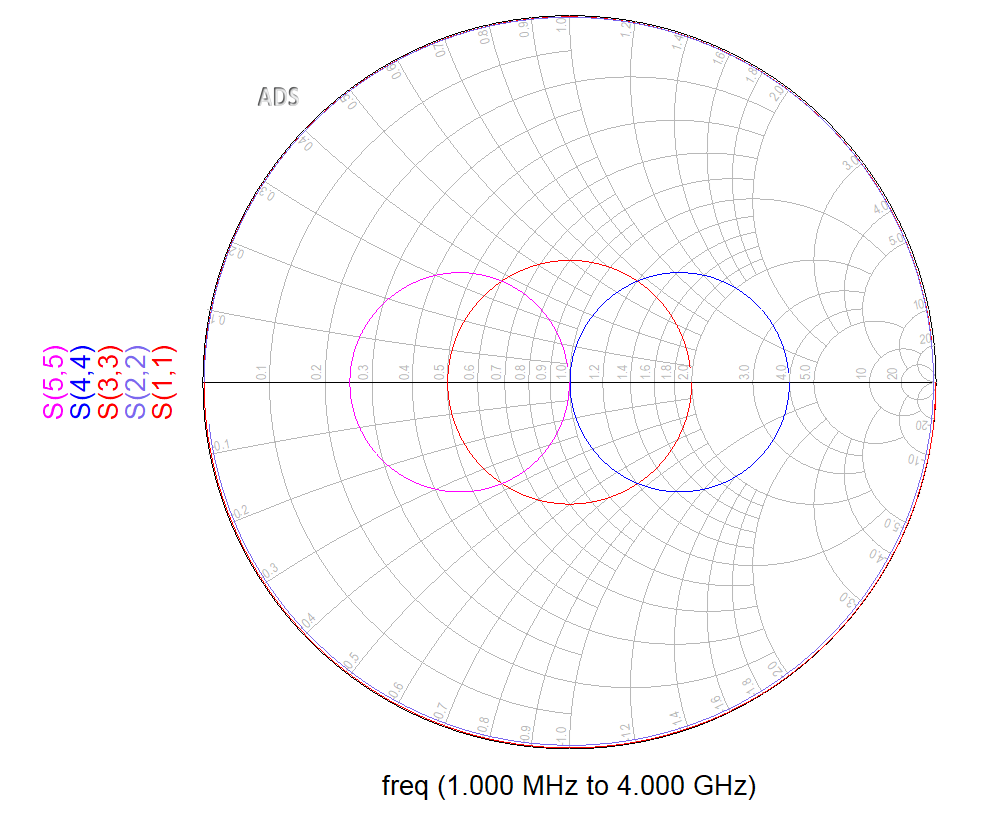
\includegraphics[width=\textwidth]{figures/schmidt.png}
        \captionof{figure}{Diagrama de Schmidt de los 5 casos estudiados.}
        \label{fig:gamma}
        \vspace{0.5cm}

        Las diferencias clave se evidenciaron en la ubicación de los puntos dentro del diagrama: cargas puramente resistivas se alinearon en el eje
        real, mientras qye condiciones extremas ocuparon los bordes del diagrama ($\Gamma$ = 1). El acoplamiento ($z_{L} = Z_{0}$)
        se situoo en el centro, sin reflexión ($\Gamma$ = 0), mientras que $Z_{L} > Z_{0}$ y $Z_{L} < Z_{0}$ mostraron $\Gamma$
        real positivo y negativo respectivamente. La ausencia de componentes reactivasmantuvo todos los casos en el eje real,
        simplificando la comparación directa de magnitudes.

        {\centering\section*{\large Conclusiones}}

        El diagrama de Schmidt es una herramienta valiosa para el análisis de circuitos de microondas, permitiendo visualizar
        relaciones complejas entre impedancias y coeficientes de reflexión. En este estudio, se observaron diferencias significativas en la
        ubicación de $\Gamma$ para diferentes escenarios de carga; la posición de $\Gamma$ en el diagrama indica la relación entre $Z_{ref}$ y $Z_{0}$,
        mientras que el radio de la circunferencia indica la magnitud de la reflexión (determinada por la relación entre $Z_{L}$ y $Z_{0}$).
        La ausencia de componentes reactivas simplificó la comparación entre los casos, permitiendo una evaluación directa de las magnitudes.
    \end{minipage}
        %\printbibliography  % Print bibliography
\end{document}